\documentclass{article}
\usepackage[paperwidth=15cm,paperheight=10cm,margin=0cm]{geometry}
\usepackage[sfdefault]{carlito}
\usepackage[T1]{fontenc}
\usepackage{tikz}
\usetikzlibrary{arrows.meta,shapes.geometric}
\definecolor{cOurs}{HTML}{4285F4}\definecolor{cOursLight}{HTML}{AECBFA}
\pagestyle{empty}
\begin{document}\noindent
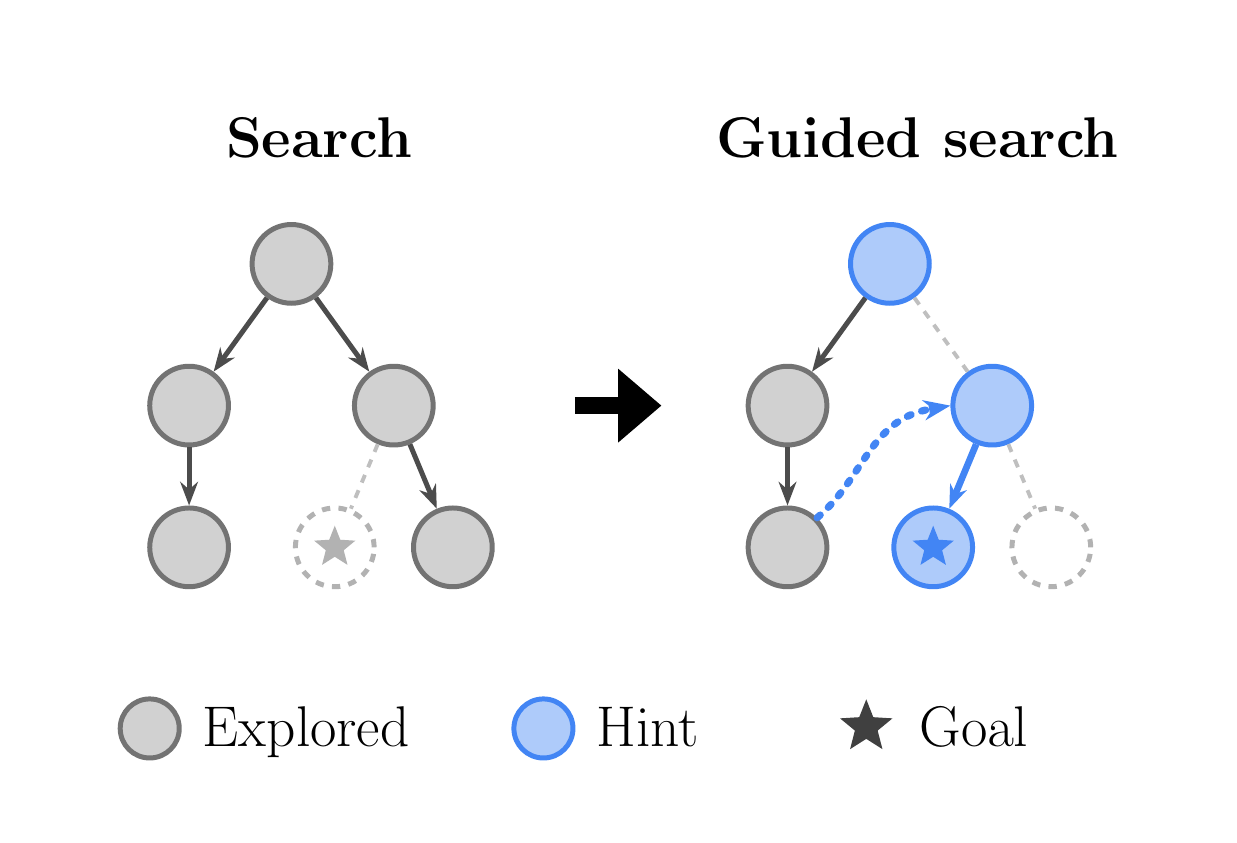
\begin{tikzpicture}[x=1cm,y=1cm,
  lab/.style={font=\fontsize{21}{24}\selectfont},
  ttl/.style={anchor=base, font=\fontsize{21}{24}\bfseries\selectfont},
  nd/.style={circle, minimum size=1.0cm, inner sep=0pt, line width=1.8pt},
  ex/.style={nd, draw=black!55, fill=black!18},
  hint/.style={nd, draw=cOurs, fill=cOursLight},
  un/.style={nd, draw=black!30, fill=white, dashed},
  e/.style={-{Stealth[length=3mm]}, line width=1.8pt, black!70},
  eh/.style={-{Stealth[length=3mm]}, line width=2.4pt, cOurs},
  eu/.style={line width=1.4pt, black!25, dashed},
  jump/.style={line width=2.6pt, cOurs, dash pattern=on 1.5pt off 4pt, line cap=round},
  goal/.style={star, star points=5, star point ratio=2.3, minimum size=0.55cm, inner sep=0pt}]
\useasboundingbox (0,0) rectangle (15,10);
\newcommand{\pos}{\coordinate (R) at (0,0); \coordinate (A) at (-1.3,-1.8); \coordinate (A1) at (-1.3,-3.6);
  \coordinate (B) at (1.3,-1.8); \coordinate (B1) at (0.55,-3.6); \coordinate (B2) at (2.05,-3.6);}
% ---- search without hints
\begin{scope}[shift={(3.35,7.0)}]\pos
  \node[ex] (r) at (R) {}; \node[ex] (a) at (A) {}; \node[ex] (a1) at (A1) {};
  \node[ex] (b) at (B) {}; \node[un] (b1) at (B1) {}; \node[ex] (b2) at (B2) {};
  \node[goal, fill=black!30] at (B1) {};
  \draw[e] (r) -- (a); \draw[e] (a) -- (a1); \draw[e] (r) -- (b); \draw[e] (b) -- (b2); \draw[eu] (b) -- (b1);
\end{scope}
\node[ttl] at (3.7,8.35) {Search};
% ---- arrow
\draw[-{Triangle[length=5.5mm, width=9mm]}, line width=6pt] (6.95,5.2) -- (8.05,5.2);
% ---- search with hints
\begin{scope}[shift={(10.95,7.0)}]\pos
  \node[hint] (r) at (R) {}; \node[ex] (a) at (A) {}; \node[ex] (a1) at (A1) {};
  \node[hint] (b) at (B) {}; \node[hint] (b1) at (B1) {}; \node[un] (b2) at (B2) {};
  \node[goal, fill=cOurs] at (B1) {};
  \draw[e] (r) -- (a); \draw[e] (a) -- (a1); \draw[eu] (r) -- (b); \draw[eh] (b) -- (b1); \draw[eu] (b) -- (b2);
  \draw[jump] (a1.north east) to[out=40, in=190] ([xshift=-2.6mm,yshift=-0.45mm]b.west);
  \draw[cOurs, line width=2.6pt, -{Stealth[length=3.4mm]}] ([xshift=-2.7mm,yshift=-0.47mm]b.west) -- (b.west);
\end{scope}
\node[ttl] at (11.3,8.35) {Guided search};
% ---- legend
\node[ex, minimum size=0.75cm] at (1.55,1.1) {}; \node[lab, anchor=base west] at (2.1,0.87) {Explored};
\node[hint, minimum size=0.75cm] at (6.55,1.1) {}; \node[lab, anchor=base west] at (7.1,0.87) {Hint};
\node[goal, fill=black!75, minimum size=0.7cm] at (10.65,1.12) {}; \node[lab, anchor=base west] at (11.2,0.87) {Goal};
\end{tikzpicture}
\end{document}
